\documentclass[12pt, a4paper]{article}

\usepackage{graphicx}
\usepackage{listings}
\usepackage{xcolor}
\usepackage{indentfirst}
\usepackage[brazilian]{babel}
\usepackage{hyphenat}

\definecolor{codegreen}{rgb}{0,0.6,0}
\definecolor{codegray}{rgb}{0.5,0.5,0.5}
\definecolor{codepurple}{rgb}{0.58,0,0.82}
\definecolor{backcolour}{rgb}{0.95,0.95,0.92}

\lstdefinestyle{colorcode}{
    backgroundcolor=\color{backcolour},   
    commentstyle=\color{codegreen},
    keywordstyle=\color{magenta},
    numberstyle=\tiny\color{codegray},
    stringstyle=\color{codepurple},
    basicstyle=\ttfamily\footnotesize,
    breakatwhitespace=false,         
    breaklines=true,                 
    captionpos=b,                    
    keepspaces=true,                 
    numbers=left,                    
    numbersep=5pt,                  
    showspaces=false,                
    showstringspaces=false,
    showtabs=false,                  
    tabsize=2
}

\lstset{style=colorcode}

\title{Relatório do Laboratório 1 \\ Segurança de Dados - Professora Denise Goya}
\author{Luiz Ricardo Bitencourt}
\date{25/02/2024}

\begin{document}

\maketitle

%%%%%%%%%%%%%%%%%%%%%%%%%%%%%%%%%%%%%%%%%%%%%%%%%%%%%%%%%%%%%%%%%%%%%%%%%%%%%%%%%%%%%%%%%%%%%%%%%%%%%%%%%%%%%%%%%%%%%%%%%%%%%%%
\section{Implementação da Cifra de Vigenère}
O laboratório propôs a criação de um programa para simular a Cifra de Vigenère, com duas funcionalidades: cifrar e decifrar. 
Abaixo, apresento os métodos criados para estas funcionalidades, mas o código completo pode ser conferido anexo.

Método para cifrar:

\begin{lstlisting}
void encrypt(char key[], char originalMessage[], char encryptedMessage[], int size){
    if (DEBUG) printf("Encrypted message (inside function): ");
    for (int i = 0; i < size; i++) {
        encryptedMessage[i] = ((((originalMessage[i] - OFFSET) + (key[i % KEY_SIZE]) - OFFSET)) % ALPHABET_SIZE) + OFFSET;
        if (DEBUG) printf("%c", encryptedMessage[i]);
    }
    if (DEBUG) printf("\n\n");
}
\end{lstlisting}

Método para decifrar:

\begin{lstlisting}
void decrypt(char key[], char mEncrypted[], char mDecrypted[], int size){
    int i;
    if (DEBUG) printf("Decrypted message (inside function): ");
    for (i = 0; i < size; i++) {
        mDecrypted[i] = (((mEncrypted[i] - OFFSET) - (key[i % KEY_SIZE] - OFFSET) + ALPHABET_SIZE) % ALPHABET_SIZE) + OFFSET;
        if (DEBUG) printf("%c", mDecrypted[i]);
    }
    if (DEBUG) printf("\n\n");
}    
\end{lstlisting}

%%%%%%%%%%%%%%%%%%%%%%%%%%%%%%%%%%%%%%%%%%%%%%%%%%%%%%%%%%%%%%%%%%%%%%%%%%%%%%%%%%%%%%%%%%%%%%%%%%%%%%%%%%%%%%%%%%%%%%%%%%%%%%%
\section{Sobre a vulnerabilidade}

Para este laboratório, foi sugerido responder ao questionamento: \textbf{por que a expressão algébrica equivale ao uso da Tabela
de Vigenère com lápis e papel?} Analisando-se o processo de cifragem, é possível construir uma tabela com as palavras nas colunas
e a chave nas linhas, realizando-se um cruzamento a cada novo caractere de forma a gerar, manualmente, a mensagem cifrada. 
Algebricamente, nota-se que cada caractere cifrado é a soma do índice do caractere da mensagem com o seu correspondente à chave,
dentro do intervalo de caracteres do alfabeto utilizado. Por isso a tabela acaba sendo um recurso facilitador na cifragem.
O processo inverso também é possível de maneira semelhante, porém montando uma tabela que considera a subtração do índice do
caractere ao índice da chave, somando-se o tamanho do alfabeto e relacionando o valor obtido a este.
A título de curiosidade, foi feito o processo de cifragem da palavra ``universidade'' usando a chave ``abc'' pelo cruzamento 
em uma tabela, conforme Figura \ref{fig:vigeneretabela}, e também usando os índices da tabela para a cifragem e decifragem manual
usando diretamente a expressão algébrica, conforme Figura \ref{fig:vigenereexpressao}.

\begin{figure}[!htpb]
    \centering
    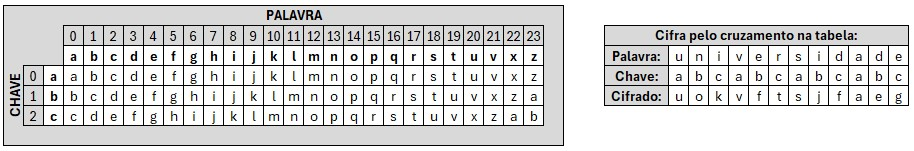
\includegraphics[scale=0.5]{img/vigenere-tabela.jpg}
    \caption{Cifragem pela tabela.}
    \label{fig:vigeneretabela}
\end{figure}

\begin{figure}[!htpb]
    \centering
    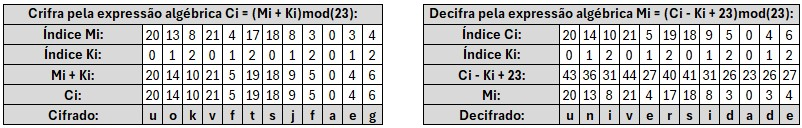
\includegraphics[scale=0.5]{img/vigenere-expres.jpg}
    \caption{Cifragem pela expressão algébrica.}
    \label{fig:vigenereexpressao}
\end{figure}

A Cifra de Vigenère é uma versão melhorada da Cifra de César, baseada na substituição de caracteres. Esta última é baseada na
adoção de uma tabela de substituição, da qual se extraem informações sobre qual caractere deve ser usado para substituir cada
caractere da mensagem original. Isso significa que pode-se chegar a mensagem original realizando-se uma análise da frequência
de caracteres, seus posicionamentos, início e final de frases, etc. Tudo isso poderia ser usado para dar indícios de quais
seriam as substituições, tornando a cifra vulnerável. Já a cifra de Vigenère usa uma tabela de substituição que varia a cada
caractere, sendo uma cifra polialfabética que usa uma chave secreta para realização das combinações e geração da mensagem
cifrada. Apesar de ser mais difícil de ser quebrada, já que a análise de frequência de caracteres não tem mais validade, como
se tem uma mesma chave podem ocorrer repetições dos padrões em intervalos regulares, o que pode dar indícios do tamanho da
chave. De posse dessa informação, é possível descobrir trechos da chave, o que possibilita decifrar trechos da informação e,
iterativamente, toda a mensagem.



\end{document}